% Template for PLoS
% Version 3.5 March 2018
%
% % % % % % % % % % % % % % % % % % % % % %
%
% -- IMPORTANT NOTE
%
% This template contains comments intended 
% to minimize problems and delays during our production 
% process. Please follow the template instructions
% whenever possible.
%
% % % % % % % % % % % % % % % % % % % % % % % 
%
% Once your paper is accepted for publication, 
% PLEASE REMOVE ALL TRACKED CHANGES in this file 
% and leave only the final text of your manuscript. 
% PLOS recommends the use of latexdiff to track changes during review, as this will help to maintain a clean tex file.
% Visit https://www.ctan.org/pkg/latexdiff?lang=en for info or contact us at latex@plos.org.
%
%
% There are no restrictions on package use within the LaTeX files except that 
% no packages listed in the template may be deleted.
%
% Please do not include colors or graphics in the text.
%
% The manuscript LaTeX source should be contained within a single file (do not use \input, \externaldocument, or similar commands).
%
% % % % % % % % % % % % % % % % % % % % % % %
%
% -- FIGURES AND TABLES
%
% Please include tables/figure captions directly after the paragraph where they are first cited in the text.
%
% DO NOT INCLUDE GRAPHICS IN YOUR MANUSCRIPT
% - Figures should be uploaded separately from your manuscript file. 
% - Figures generated using LaTeX should be extracted and removed from the PDF before submission. 
% - Figures containing multiple panels/subfigures must be combined into one image file before submission.
% For figure citations, please use "Fig" instead of "Figure".
% See http://journals.plos.org/plosone/s/figures for PLOS figure guidelines.
%
% Tables should be cell-based and may not contain:
% - spacing/line breaks within cells to alter layout or alignment
% - do not nest tabular environments (no tabular environments within tabular environments)
% - no graphics or colored text (cell background color/shading OK)
% See http://journals.plos.org/plosone/s/tables for table guidelines.
%
% For tables that exceed the width of the text column, use the adjustwidth environment as illustrated in the example table in text below.
%
% % % % % % % % % % % % % % % % % % % % % % % %
%
% -- EQUATIONS, MATH SYMBOLS, SUBSCRIPTS, AND SUPERSCRIPTS
%
% IMPORTANT
% Below are a few tips to help format your equations and other special characters according to our specifications. For more tips to help reduce the possibility of formatting errors during conversion, please see our LaTeX guidelines at http://journals.plos.org/plosone/s/latex
%
% For inline equations, please be sure to include all portions of an equation in the math environment.  For example, x$^2$ is incorrect; this should be formatted as $x^2$ (or $\mathrm{x}^2$ if the romanized font is desired).
%
% Do not include text that is not math in the math environment. For example, CO2 should be written as CO\textsubscript{2} instead of CO$_2$.
%
% Please add line breaks to long display equations when possible in order to fit size of the column. 
%
% For inline equations, please do not include punctuation (commas, etc) within the math environment unless this is part of the equation.
%
% When adding superscript or subscripts outside of brackets/braces, please group using {}.  For example, change "[U(D,E,\gamma)]^2" to "{[U(D,E,\gamma)]}^2". 
%
% Do not use \cal for caligraphic font.  Instead, use \mathcal{}
%
% % % % % % % % % % % % % % % % % % % % % % % % 
%
% Please contact latex@plos.org with any questions.
%
% % % % % % % % % % % % % % % % % % % % % % % %

\documentclass[10pt,letterpaper]{article}
\usepackage[top=0.85in,left=2.75in,footskip=0.75in]{geometry}

% amsmath and amssymb packages, useful for mathematical formulas and symbols
\usepackage{amsmath,amssymb}

% Use adjustwidth environment to exceed column width (see example table in text)
\usepackage{changepage}

% Use Unicode characters when possible
\usepackage[utf8x]{inputenc}

% textcomp package and marvosym package for additional characters
\usepackage{textcomp,marvosym}

% cite package, to clean up citations in the main text. Do not remove.
\usepackage{cite}

% Use nameref to cite supporting information files (see Supporting Information section for more info)
\usepackage{nameref,hyperref}

% line numbers
\usepackage[right]{lineno}

% ligatures disabled
\usepackage{microtype}
\DisableLigatures[f]{encoding = *, family = * }

% color can be used to apply background shading to table cells only
\usepackage[table]{xcolor}

% array package and thick rules for tables
\usepackage{array}

\usepackage{dcolumn}

% create "+" rule type for thick vertical lines
\newcolumntype{+}{!{\vrule width 2pt}}

% create \thickcline for thick horizontal lines of variable length
\newlength\savedwidth
\newcommand\thickcline[1]{%
  \noalign{\global\savedwidth\arrayrulewidth\global\arrayrulewidth 2pt}%
  \cline{#1}%
  \noalign{\vskip\arrayrulewidth}%
  \noalign{\global\arrayrulewidth\savedwidth}%
}

% \thickhline command for thick horizontal lines that span the table
\newcommand\thickhline{\noalign{\global\savedwidth\arrayrulewidth\global\arrayrulewidth 2pt}%
\hline
\noalign{\global\arrayrulewidth\savedwidth}}


% Remove comment for double spacing
%\usepackage{setspace} 
%\doublespacing

% Text layout
\raggedright
\setlength{\parindent}{0.5cm}
\textwidth 5.25in 
\textheight 8.75in

% Bold the 'Figure #' in the caption and separate it from the title/caption with a period
% Captions will be left justified
\usepackage[aboveskip=1pt,labelfont=bf,labelsep=period,justification=raggedright,singlelinecheck=off]{caption}
\renewcommand{\figurename}{Fig}

% Use the PLoS provided BiBTeX style
\bibliographystyle{plos2015}

% Remove brackets from numbering in List of References
\makeatletter
\renewcommand{\@biblabel}[1]{\quad#1.}
\makeatother



% Header and Footer with logo
\usepackage{lastpage,fancyhdr,graphicx}
\usepackage{epstopdf}
%\pagestyle{myheadings}
\pagestyle{fancy}
\fancyhf{}
%\setlength{\headheight}{27.023pt}
%\lhead{\includegraphics[width=2.0in]{PLOS-submission.eps}}
\rfoot{\thepage/\pageref{LastPage}}
\renewcommand{\headrulewidth}{0pt}
\renewcommand{\footrule}{\hrule height 2pt \vspace{2mm}}
\fancyheadoffset[L]{2.25in}
\fancyfootoffset[L]{2.25in}
\lfoot{\today}

%% Include all macros below

\newcommand{\lorem}{{\bf LOREM}}
\newcommand{\ipsum}{{\bf IPSUM}}

%% END MACROS SECTION


\begin{document}
\vspace*{0.2in}

% Title must be 250 characters or less.
\begin{flushleft}
{\Large
\textbf\newline{The role of education, religiosity and development on support for violent practices among Muslims in thirty-five countries} % Please use "sentence case" for title and headings (capitalize only the first word in a title (or heading), the first word in a subtitle (or subheading), and any proper nouns).
}
\newline
% Insert author names, affiliations and corresponding author email (do not include titles, positions, or degrees).
%\\
%Aaron Gullickson\textsuperscript{1*},
%Sarah Ahmed\textsuperscript{1}
%\\
%\bigskip
%\textbf{1} Department of Sociology, University of Oregon, Eugene, OR, USA
%\\
%\bigskip

% Insert additional author notes using the symbols described below. Insert symbol callouts after author names as necessary.
% 
% Remove or comment out the author notes below if they aren't used.
%
% Primary Equal Contribution Note
%\Yinyang These authors contributed equally to this work.

% Additional Equal Contribution Note
% Also use this double-dagger symbol for special authorship notes, such as senior authorship.
%\ddag These authors also contributed equally to this work.

% Current address notes
%\textcurrency Current Address: Dept/Program/Center, Institution Name, City, State, Country % change symbol to "\textcurrency a" if more than one current address note
% \textcurrency b Insert second current address 
% \textcurrency c Insert third current address

% Deceased author note
%\dag Deceased

% Group/Consortium Author Note
%\textpilcrow Membership list can be found in the Acknowledgments section.

% Use the asterisk to denote corresponding authorship and provide email address in note below.
%* aarong@uoregon.edu

\end{flushleft}
% Please keep the abstract below 300 words
\section*{Abstract}
Despite widespread scholarly interest in values and attitudes among
Muslim populations, relatively little work has focused on specific
attitudes popularly thought to indicate anti-modern or anti-liberal
tendencies within Islam. In this article, we use data from the Pew
Research Center from 2008-2012 to examine support for violent practices
among Muslims in thirty-five countries. Support for violent practices is
defined by three questions on the acceptability of killing apostates,
the stoning of adulterers, and severe corporal punishment for thieves.
Using multilevel models that capture country-level variability, we
analyze the relationship between support for violent practices and
education, religiosity, and development. In general, we find that
support for violent practices is less common among individuals with more
education and less religiosity and who come from more developed
countries. However, when we examine variation across countries, we see
evidence of substantial heterogeneity in the association of education
and religiosity with support for violent practices. We find that
education and religiosity are less liberalizing in less liberal
countries. Furthermore, there is no association between the effects of
education and religiosity within a country. We discuss the implications
of these findings more broadly based on prior work on liberal value
systems in mostly Western countries. Overall, the variation we observe
across countries calls into question a civilizational approach to
studying values among Muslim populations and points to a more nuanced
multiple modernities approach.

% Please keep the Author Summary between 150 and 200 words
% Use first person. PLOS ONE authors please skip this step. 
% Author Summary not valid for PLOS ONE submissions.   
%\section*{Author summary}
%Lorem ipsum dolor sit amet, consectetur adipiscing elit. Curabitur eget porta erat. Morbi consectetur est vel gravida pretium. Suspendisse ut dui eu ante cursus gravida non sed sem. Nullam sapien tellus, commodo id velit id, eleifend volutpat quam. Phasellus mauris velit, dapibus finibus elementum vel, pulvinar non tellus. Nunc pellentesque pretium diam, quis maximus dolor faucibus id. Nunc convallis sodales ante, ut ullamcorper est egestas vitae. Nam sit amet enim ultrices, ultrices elit pulvinar, volutpat risus.

\linenumbers

% Use "Eq" instead of "Equation" for equation citations.
\section*{Introduction}

In a viral appearance on the HBO Show ``Real Time with Bill Maher'' in
2014, actor Ben Affleck became embroiled in an unexpected debate with
host Bill Maher and fellow guest, Sam Harris, over the allegedly
authoritarian and violent tendencies of Islamic doctrine
\cite{casey_real_2014}. Harris, one of the leading figures in the New
Atheist movement, argued that Islam ``at this moment is the motherlode
of bad ideas.'' To support this view, Maher offered data from a recent
poll of Muslims worldwide conducted by the Pew Research Center which
showed that ``like 90\%'' of Egyptian Muslims supported death as a
punishment for leaving the faith.

Although Maher's figure was factually correct, the statistic is
nonetheless misleading. Egyptian Muslims were more supportive of this
statement than Muslims in any other country in the Pew study. In
contrast, only 0.8\% of Muslims in Kazakhstan felt similarly. Among the
more than thirty countries in the cited Pew survey as well as a similar
one conducted in sub-Saharan Africa, the level of support among Muslims
for killing apostates varies uniformly between these two extremes.
Substantial variation rather than strict orthodoxy is the key to
understanding Muslim responses to this question. For social scientists,
this variation then begs a further question - why do Muslims vary so
much in their support for such ``bad'' ideas?

In this article, we take up this question with a more formal analysis of
the Pew data. The data were collected between 2008-12 on Muslims in
thirty-five countries representing roughly sixty-five percent of the
global Muslim population. From this data, we develop a value construct
measuring support for violent practices from three questions on the
acceptability of killing apostates, the stoning of adulterers, and
severe corporal punishment for thieves. Following prior work on the
impact of modernization and development on liberal values in mostly
Western contexts, our analysis focuses on the relationship between this
value construct, education, religiosity, and development.

Our analysis builds on an extensive literature on values and attitude
among Muslims, and complements prior research in two important ways.
First, we address specific attitudes that have never been examined in
scholarly work, despite their prominence in popular discussions of Islam
in the West. Most prior research focuses either on attitudes regarding
universalistic and abstract concepts such as support for democracy,
political violence, and gender equality, or relies upon large aggregate
indices that are driven by a multitude of specific attitudes ranging
from acceptance of abortion to whether respondents would be willing to
sign a petition \cite{inglehart_worldviews_2007}.

A focus on universalistic attitudes, however, provides little insight
into the specific attitudes and values that differentiate cultural and
religious groups. For example, whether a respondent is willing to sign a
petition or is supportive of democracy in the abstract may tell us
little to nothing about how that respondent feels toward the mandate
that apostates should be killed. Yet, the justifiability of killing
apostates is a topic that both divides Muslims internally and
distinguishes Muslims from other religious groups. It is not simply that
Muslims feel differently on this issue in comparison to other religious
groups, but rather that the question itself is only intelligible among
Muslims.

Second, the large sample of countries here allows us to more
systematically examine country-level variation than has been possible in
much of the prior work on value systems in Muslim populations. While
classic modernization theory expected a fairly uniform pattern of
modernization, contemporary scholars expect greater heterogeneity in
this process \cite{eisenstadt_civilizational_2001}. Some have even
suggested that change in cultural systems -- including values and
attitudes -- may be largely unconnected to processes of modernization
and development \cite{huntington_clash_1996}. To better understand this
heterogeneity, we use multilevel models that provide information about
country-level variation in support for violent practices and
country-level variation in the association between support for violent
practices and education and religiosity. We argue that the pattern of
variation at the country level provides insight into the role of
educational and religious institutions in the process of value change.

When we pool results across countries, our analysis largely supports the
expectations of modernization theory. Support for violent practices is
less common among individuals with more education and less religiosity
and who come from more developed countries. However, when we examine
variation across countries, we see evidence of substantial heterogeneity
in the effects of education and religiosity on support for violent
practices. In both cases, we find that the association between
education/religiosity is less liberalizing in countries that are more
supportive of violent practices overall, suggesting that the role of
educational and religious institutions shifts with changes in the larger
society. Furthermore, we find little association between the effects for
education and religiosity themselves, suggesting that idiosyncratic
county-level factors operate independently on religious and educational
institutions.

\section*{Background}

Prior work on values and attitudes in Muslim populations has focused on
a variety of such attitudes including support for democracy
\cite{jamal_attitudes_2008, ciftci_modernization_2010, ciftci_secularislamist_2013},
political violence\cite{mousseau_urban_2011, berger_foreign_2014},
women's rights \cite{inglehart_true_2003}, and fundamentalism
\cite{moaddel_religious_2018}. While a summary of this work is beyond
the scope of this article, such studies are often framed around
modernization theory and its closely related cousin, secularization
theory, as well as critiques of these theories
\cite{jamal_reassessing_2006, moaddel_introduction_2007, ciftci_modernization_2010}.

Modernization theory treats cultural and value change as largely a
by-product of structural development
\cite{lerner_passing_1958, parsons_social_1964, inkeles_becoming_1974}.
Industrialization and economic growth bring about greater
differentiation in the occupational workforce, urbanization, and higher
standards of living \cite{rostow_stages_1960}. All of these factors
contribute to a shift from conservative and authoritarian values to
liberal values that promote individual autonomy and self-determination
\cite{parsons_social_1964}. Concomitantly, rationalization,
individualism, and cultural pluralism reduce the significance of
religious institutions in favor of secular institutions, diminishing the
role of religion in social life
\cite{wilson_religion_1966, bruce_secularization_2011, emerson_rise_2006}.

For this article, we focus on two important themes within this
framework. First, scholars often treat education and religiosity as key
variables at the individual level connected to processes of
modernization and value change \cite{scheepers_education_2002}. Second,
contemporary critiques of modernization theory have often pointed to the
heterogeneity and variation in the experience of development across
countries rather than its uniformity and standardization
\cite{smith_future_2008}.

\subsection*{The role of education and religiosity on values}

Education is often seen as a crucial fulcrum at the individual level for
processes of modernization
\cite{meyer_effects_1977, chabbott_development_2000, depaepe_educationalization_2008}.
In terms of value change, research has repeatedly shown that education
is positively related to liberal values
\cite{hyman_education_1979, bobo_education_1989, weakliem_effects_2002, kingston_why_2003}.

While these results are broadly consistent with modernization theory,
significant debate has persisted on how to understand this finding. The
development perspective holds that education is linked to fundamental
cognitive changes in the way people view the world that leads to more
tolerance and less authoritarianism
\cite{adorno_authoritarian_1950, mcclosky_dimensions_1983}. On the
other hand, the socialization perspective argues that educational
institutions socialize individuals to the prevailing norms of a society
\cite{selznick_tenacity_1969, jackman_education_1984, phelan_education_1995}.
Therefore, the liberalizing effects of education will only exist in
countries where liberal values are commonplace. Consistent with the
socialization perspective, cross-national results in Western countries
show that the positive effect of education is greatest in countries with
more liberal values overall \cite{weil_variable_1985}.

Social scientists have often treated religiosity as the anti-modern
counterweight to education \cite{schwadel_explaining_2015}. High levels
of religiosity are seen to indicate commitments to conservative and
authoritarian values
\cite{rokeach_part_1969, rokeach_part_1969a, wilcox_evangelicals_1990}.
Although there is significant heterogeneity across countries, research
has shown that religious identification tends to be associated with
support for right-wing parties and more conservative attitudes
\cite{wilcox_evangelicals_1990, kelley_class_1995, scheepers_religion_1998, karpov_religiosity_2002, norris_sacred_2011}.

However, the relationship between religiosity and conservative values
may be partially tautological depending on how religiosity is defined.
Given that the core religious texts of the major Western religions are
frequently conservative and authoritarian, it is not surprising that
strong believers with a tendency for theological literalism would
themselves be more conservative and authoritarian. Therefore, in
analyzing the effect of religiosity on values and attitudes, it is
imperative to distinguish the effects of theological conservatism and
literalism from the effects of variables that measure how important
religion and religious practices are in a person's life.

Although less widely acknowledged than for the case of education, the
effect of religiosity may similarly be mediated by the role that
religious institutions play as socialization agents
\cite{scheepers_education_2002}. In particular, religious institutions
may respond to the prevailing norms and beliefs in a society in one of
two ways. Greater liberalism within a society may dampen the
conservative effect of religiosity on liberal values or it may
alternatively provoke a greater defense of religious values and increase
the association between religiosity and conservative values
\cite{kelley_national_1997}.

\subsection*{Heterogeneity and multiple modernities}

Modernization theorists have viewed modernization as a fundamental
process that would evolve similarly across countries, ultimately
producing a global cosmopolitan society through the broad convergence in
social and cultural systems \cite{fukuyama_end_1992}. Many scholars
today criticize this view for privileging the historical experience of
the West as a universal model. These ``multiple modernities'' scholars
argue that while modernity will likely lead to changes in social and
cultural systems, these changes will materialize in multiple dissimilar
and non-convergent forms because countries develop within various
historical and cultural contexts
\cite{hefner_multiple_1998, eisenstadt_multiple_2000, kamali_multiple_2006, casanova_cosmopolitanism_2011}.

In the present study, consideration of such heterogeneity is relevant to
studying values in Muslim populations in two ways. First, the
``civilizational'' argument proposed by Samuel Huntington
suggests that heterogeneity across countries will largely correspond to
civilizational blocs defined primarily along religious lines \cite{huntington_clash_1996}. According
to Huntington, Western liberal traditions such as individualism, support
for pluralism, and secularism are not intrinsic to the process of
modernity but rather a specific inheritance of Western civilization
\cite{huntington_clash_1996}. If this is the case, then
we should not expect to see that development, education, and religiosity
have the same effect on values and attitudes in Muslim societies as
those observed elsewhere.

Specifically, Huntington argued that the primary agents for the
contemporary rise of Islamic fundamentalism were an urban and educated
middle class \cite{huntington_clash_1996}. Rapid economic
growth and urbanization dislocate individuals from traditional
structures of social support and this dislocation is experienced most
intensely by upwardly mobile, young, urban, and educated individuals.
Therefore, contrary to research primarily in Western contexts showing a
positive relationship between liberal values and education, Huntington
expected a negative relationship in Muslim societies.

Second, and contrary to the expectation of both classic modernization
theory and the civilizational argument, we may observe significant
variation in how educational and religious institutions affect values
across Muslim countries. These differences may reflect a wide variety of
societal influences, some of which are historical and idiosyncratic.
Nonetheless the patterning of such variation across countries may be
informative. The expectations of socialization theory discussed above
are one example of such patterning. We discuss further expectations
below.

\section*{Analytical approach and theoretical expectations}

Using the Pew data detailed below, we build a model that can
simultaneously measure the effects of education, religiosity, and
development on support for violent practices and account for
heterogeneity in these effects across countries. Specifically, we use a
random intercept and random slope multilevel model, in which the
intercepts and the slopes for the educational attainment and religiosity
variables are allowed to vary across countries. Our general model
specification is:

\[y_{ij}=\beta_{0j}+\beta_{1j}(\texttt{religiosity}_{ij})+\beta_{2j}(\texttt{education}_{ij})+\sum_{k=1}^K \lambda_kx_{ijk}+\epsilon_{ij}\]

where \(y_{ij}\) is the score on the measure of support for violent
practices (detailed below) for the \(i\)th respondent in the \(j\)th
country. The intercept \(\beta_{0j}\), and the two slopes of
\(\beta_{1j}\) and \(\beta_{2j}\) on religiosity and education,
respectively, are allowed to vary by country. The model also includes
\(K\) additional independent control variables \(x_{ijk}\) that are not
allowed to vary by country. \(\epsilon_{ij}\) is an individual-level
error term.

To complete the multilevel model structure, the three country-varying
parameters have their own linear equations:

\[\beta_{0j}=\gamma_{01}+\gamma_{02}\texttt{development}_j+\delta_j\]
\[\beta_{1j}=\gamma_{11}+\gamma_{12}\texttt{development}_j+\eta_j\]
\[\beta_{2j}=\gamma_{21}+\gamma_{22}\texttt{development}_j+\tau_j\]

The structure shown here is for the fullest model in which we include a
country-level measure of development (detailed below) that predicts the
intercept and the two slopes. The \(\gamma_{02}\) term measures the
association between development and average support for violent
practices in a country. The \(\gamma_{12}\) and \(\gamma_{22}\) terms
measure how development in a country affects the individual-level
relationship between support for violent practices and either education
or religiosity, respectively.

The error terms \(\delta_j\), \(\eta_j\) and \(\tau_j\) are
country-level random effects that measure country-level heterogeneity in
terms of the intercept and two slopes. Because the correlation of these
random effects is important for our understanding of this heterogeneity
across countries, we place no restrictions on the correlation between
these error terms in the estimation of the model.

Given the model outlined above, we develop several expectations about
the estimates it will produce. These expectations relate to several
different parameters in the model. First, we lay out the expectations of
the effects of development at the country level (\(\gamma_{02}\)) as
well as the average effects of religiosity (\(\gamma_{11}\)) and
educational attainment (\(\gamma_{21}\)) across countries. Modernization
theory expects that overall development at the country level and
educational attainment at the individual level will be negatively
associated with support for violent practices, while religiosity will be
positively associated with support for violent practices.

Second, we also consider how development might affect the relationship
between support for violent practices and religiosity (\(\gamma_{12}\))
or educational attainment (\(\gamma_{22}\)). We consider two
possibilities for each variable. First, modernization may produce a
``flattening'' effect in which overall development reduces the
association as individuals become more liberal regardless of education
or religiosity. Alternatively, modernization may produce a
``steepening'' effect in which the association gets larger as
development increases and differences in values grow in magnitude
between individuals of different educational attainment or religiosity.

Finally, we explore the heterogeneity in the effects of education and
religiosity across countries by an examination of the correlation
between the random components of the model. These random components
provide estimates of how specific countries deviate from the global
averages. We analyze these correlations in two ways. First, we analyze
how the country-level variation in the association between support for
violent practices and religiosity (\(\eta_j\)) or educational attainment
(\(\tau_j\)) is correlated with the overall average level of support for
violent practices within that country (\(\delta_j\)). These correlations
tell us the degree to which these associations increase or decrease with
the overall sentiment of the country. They therefore offer a test of the
socialization hypothesis which would expect a positive correlation. If
this is the case, it suggests that educational and religious
institutions move in step with popular attitudes.

Second, we analyze the correlation between the religiosity (\(\eta_j\))
or educational attainment (\(\tau_j\)) random effects themselves. This
correlation tells us the degree to which unmeasured factors producing
heterogeneity in these effects across countries operate similarly or
differently on educational and religious institutions. We consider three
possibilities for this correlation. If the correlation is positive, then
we observe a process of synchronicity in which educational and religious
institutions are responding in the same way to other societal
influences. Alternatively, if the correlation is negative, then we
observe a process of polarization between education and religious
institutions, in which other societal influences push educational and
religious institutions in opposite directions. A third possibility is
that the correlation is zero, suggesting that the societal changes
affecting these institutions operate in independent and unconnected
ways.

\section*{Materials and methods}

Data for this analysis come primarily from two cross-national surveys
conducted by the Pew Research Center's Religion and Public Life project.
The first survey, \emph{Tolerance and Tension: Islam and Christianity in
Sub-Saharan Africa}, sampled more than 25,000 respondents in nineteen
countries in sub-Saharan Africa in 2008-2009. The second survey,
\emph{The World's Muslims: Religion, Politics and Society}, sampled more
than 30,000 Muslim respondents in twenty-six countries throughout the
world in 2011-2012. The questionnaires for the surveys are very similar,
although additional questions were added and some other questions were
re-worded in the second survey. We focus our analysis only on questions
that are consistent across both surveys.

We combine Muslim respondents from these surveys together to construct
our full analytical dataset. Five sub-Saharan African countries
(Democratic Republic of Congo, Botswana, Rwanda, South Africa, and
Zambia) were excluded from analysis because of minuscule (2\% or less)
Muslim populations. Four other countries were excluded because key
questions for the analysis were not asked in those countries (Iran,
Morocco, Mozambique, and Uzbekistan). Finally, Thailand was excluded
because the sample was not nationally representative. Fig~\ref{fig1} shows a
map of the countries included in our analysis with shading by the
percent Muslim in each country. The countries in the sample cover all
regions of the world with substantial Muslim populations. In total, we
use data from 35 countries and 35,400 respondents. The average sample
size per country was 1,011 respondents with a minimum size of 245
respondents in Cameroon and a maximum size of 1,918 respondents in
Bangladesh.

\begin{figure}[!h]
%\begin{adjustwidth}{-2.25in}{0in}
\centering
%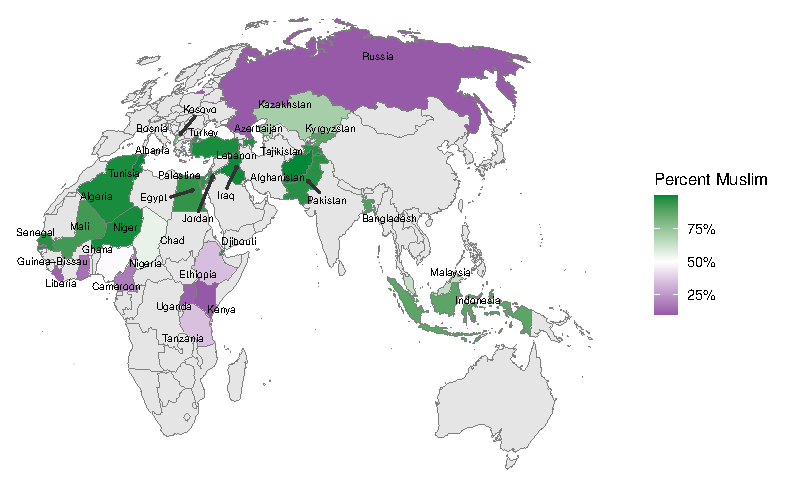
\includegraphics{figures/fig1.eps}
\caption{Map showing countries included in the analysis by percent
Muslim. Mollweide projection used to preserve area proportions.}
\label{fig1}
%\end{adjustwidth}
\end{figure}

Because the country-level surveys were designed to be nationally
representative, the data should be representative of within-country
populations, but not necessarily the global Muslim population.
Collectively, the countries in the sample roughly account for sixty-five
percent of the global Muslim population
\cite{pewforumonreligionandpubliclife_global_2012}, but some important
countries both symbolically (e.g.~Saudi Arabia, Iran) and by population
weight (e.g.~India) are absent.

Several variables used in this analysis are constructs made up of
multiple individual items, including the dependent variable and the
measure of religiosity. All constructs were developed through an
exploratory factor analysis that identified points of separation and
correlation between items.

\subsection*{Measuring support for violent practices}

We develop our measures of support for violent practices based on
multiple questions that were fielded in both surveys. Respondents were
asked yes/no questions for whether they favored (a) the death penalty
for people who leave Islam, (b) harsh punishments like whipping and
cutting off hands for crimes like theft and robbery, and (c) stoning
people who committed adultery. These three measures were highly
correlated with one another (Cronbach's \(\alpha=0.83\)) and exploratory
factor analysis indicated that a single scale worked well for all three
variables. We also considered a likert-scale question on the
justifiability of violence against civilians in defense of religion, but
this variable had a much weaker correlation with the three other
measures and so we dropped it from analysis.

Fig~\ref{fig2} shows the average level of support by country for the three
items that make up our measure of support for violent practices.
Countries tend to have similar levels of support for all items within
the construct, but the variation across countries is substantial.
Support for these values ranges from virtually no support in countries
such as Azerbaijan and Kazakhstan to nearly universal support in
countries such as Afghanistan and Egypt.

\begin{figure}[!h]
%\begin{adjustwidth}{-2.25in}{0in}
\centering
%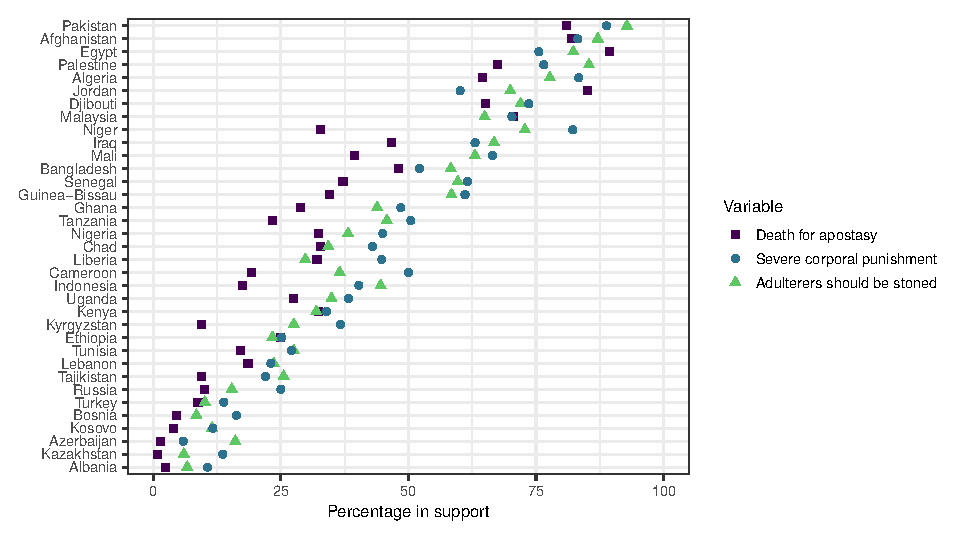
\includegraphics{figures/fig2.eps}
\caption{Dotplot of percentage of Muslim respondents who support three
different questions measuring support for violent practices for the
violation of norms. Countries are ordered from lowest to highest average
level of support across all three questions.}
\label{fig2}
%\end{adjustwidth}
\end{figure}

We constructed the dependent variable for our models by counting the
number of favorable responses to each question and then re-scaling this
tally to have a mean of zero and a standard deviation of one.

\subsection*{Measuring development}

At the country-level, we considered two different possibilities for a
measure of overall development. Gross domestic product (GDP) per capita
is often used as a purely economic measure of the level of development.
On the other hand, the Human Development Index (HDI), produced by the
United Nations Development Program, offers a more holistic measure of
development. The HDI considers three separate components in its overall
measure: life expectancy at birth, overall educational attainment, and
gross national income per capita. These three components are combined
into a single composite index.

These two measures are highly correlated among the countries used in the
analysis (\(r=0.78\)). All models reported here use the HDI. We chose
the HDI as our primary measure of development because it allows us to
parsimoniously capture mutiple dimensions of development. As a
sensitivity analysis, we constructed identical models with a logged GDP
per capita measure. The results were similar, although the logged GDP
variable tended to produce slightly smaller overall effects than HDI.
The models from this sensitivity analysis are available in the
\nameref{S1_Appendix}.

\subsection*{Independent variables}

Education is a key measure in our analysis, but the categories used for
educational attainment are country-specific, making it challenging to
include in a cross-national analysis. Educational attainment was
reported as a three-category system for the sub-Saharan African
countries and relative to country-specific educational systems for the
remaining countries. These country-specific systems ranged from a high
of twelve distinct categories to a low of five distinct categories. We
harmonized these measures by creating a quantile score based on the
distribution of the educational attainment variable within each country.
Each respondent was assigned a midpoint value on the quantile score
between their given level of education and the next lowest level (or
zero when the respondent was in the lowest category). This quantile
score measures a respondent's relative position on the distribution of
education within a country. We also considered a three-category measure
of absolute educational attainment consisting of no secondary education,
at least some secondary education, and post-secondary education that
could be used for all countries. Sensitivity tests showed that these
models produced similar results, but the BIC model fit statistics
strongly preferred the educational quantile measure. Full results are
available in the \nameref{S1_Appendix}.

We measure each respondent's religiosity using a concept that combines
the experiential and ritualistic dimensions of Glock and Stark's framework \cite{glock_religion_1965}. Our goal is to isolate the
importance of religion in a person's daily life as measured by their
personal experience and practice of it from specific ideological beliefs
and knowledge about the religion. We measure religiosity with a
three-item construct including a question on the importance of religion
in a person's life, the frequency of mosque attendance, and the
frequency of prayer. Across the entire sample, this three item construct
had a Cronbach's \(\alpha\) of 0.68. Mosque attendance has been
criticized by some scholars as an inappropriate Western import for
measuring religiosity among Muslims \cite{el-menouar_five_2014}.
However, sensitivity tests suggested that mosque attendance had similar
effects on outcomes as other measures of religiosity when we examined
the separate effect of each variable and we therefore retain it. These
results are available in the \nameref{S1_Appendix}.

Prior research has shown that religiosity is positively associated with
theological literalism, conservativism, and fundamentalism among Muslims
\cite{moaddel_religious_2018}. Individuals with more literal and
theologically conservative beliefs are likely to have more anti-liberal
values simply because some of the measures used for the dependent
variable can be argued to have scriptural justification. To control for
this potential confounding influence in our analysis, we tested a
separate construct that measured theological conservatism and literalism
in a person's actual beliefs. We considered questions on whether a
person must believe in god to be moral, whether Islam is the one true
faith, and whether there was only one way to interpret religious
teachings. However, these questions did not hold up well as a single
construct (Cronbach's \(\alpha=0.38\)). Therefore, to capture
theologically conservative beliefs and practices, we included all three
questions as separate independent variables in our models.

We include a variety of other individual-level variables in all models.
We include variables for the age (five-year brackets), gender, income,
and urbanicity of the respondent. Income was reported in loosely defined
quartiles (i.e.~four categories from ``low'' to ``high'') for the
sub-Saharan African countries and brackets that were specific to each
national currency for remaining countries and so we use a method
identical to that for education to create income quantile scores. The
country-specific income brackets ranged from a high of seventeen
distinct categories to a low of five distinct brackets.

We also include a measure of the respondent's self-reported
denomination. The primary division here is between Sunni and Shia, but
many respondents also identified in a non-denominational way
(e.g.~``just a Muslim'') which we retain as a separate category. We
combine all other denominations into a single ``other'' category. A
separate item asked respondents whether they identified with any Sufi
orders. We code this as a binary variable that is distinct from the
denominational categories.

We also control for non-religious ideological views. We constructed an
index of socially conservative views based on the respondent's answers
regarding the acceptability of seven stigmatized behaviors (drinking
alcohol, euthanasia, suicide, abortion, prostitution, premarital sex,
and homosexuality; Cronbach's \(\alpha=0.76\)). We also combine two
questions that gauge respondents' attitudes toward Western movies,
music, and television into an anti-Westernization scale. Finally, we
include questions on whether religion is in conflict with modernity, and
whether the country would be better off with a strong leader rather than
a democratic government.

\subsection*{Multiple imputation}

We use multiple imputation to address missing values in the dataset. We
imputed five complete datasets using multivariate imputation by chained
equations \cite{buuren_mice_2011}. We generally did not impute values
when a question was missing because it was not asked in a particular
country, but we made two exceptions to this rule. Questions regarding
the moral acceptability of prostitution, premarital sex, and
homosexuality were not asked in Afghanistan and the two questions about
the morality of western movies, music, and television were not asked in
Lebanon. In both of these cases, we imputed values in order to maximize
country sample size. The percentage of values imputed ranged from a high
of 11.4\% for the question on whether religion was in conflict with
modernity to 0.7\% for the respondent's age. We included dependent
variables in the imputation procedure, but drop cases that were missing
on the dependent variable. After this exclusion, the sample size of our
anlalytical dataset is 31,528 respondents.

\subsection*{Scaling variables}

To facilitate comparisons between variables in the models, all
quantitative variables have been re-centered on the mean and re-scaled.
The dependent variable has been divided by its standard deviation.
Independent variables have been divided by twice their standard
deviation. The estimated effects of quantitative variables shown
throughout this article can be interpreted as the expected change in
standard deviations of the dependent variable for an increase of two
standard deviations in the independent variable. Dividing by twice the
standard deviation makes the slopes of quantitative variables in linear
models roughly comparable to the effects of categorical dummy variables
\cite{gelman_scaling_2008}.

% Results and Discussion can be combined.
\section*{Results}

Table~\ref{tab1} shows the results of three multilevel models predicting support for violent practices. Model 1 includes only individual level variables. Model 2 adds in the country-level Human Development Indicator (HDI) as a predictor of average support for violent practices in a country. Model 3 additionally allows HDI to be a predictor of the association between religiosity/education and support for violent practices within a country.

\begin{table}
\begin{adjustwidth}{-2.25in}{0in}
\caption{Results from multilevel models predicting support for violent practices for violating norms among Muslims.}
\begin{center}
\begin{tabular}{l D{)}{)}{13)3} D{)}{)}{13)3} D{)}{)}{13)3}}
\hline
 & \multicolumn{1}{c}{Model 1} & \multicolumn{1}{c}{Model 2} & \multicolumn{1}{c}{Model 3} \\
\hline
Intercept                             & -0.088 \; (0.086)       & -0.119 \; (0.086)       & -0.104 \; (0.086)       \\
Religiosity                           & 0.249 \; (0.033)^{***}  & 0.239 \; (0.033)^{***}  & 0.240 \; (0.033)^{***}  \\
Education quantile                    & -0.062 \; (0.023)^{**}  & -0.064 \; (0.023)^{**}  & -0.059 \; (0.022)^{**}  \\
Income quantile                       & -0.006 \; (0.010)       & -0.005 \; (0.010)       & -0.006 \; (0.010)       \\
Age 25-29                             & 0.010 \; (0.014)        & 0.011 \; (0.014)        & 0.010 \; (0.014)        \\
Age 30-34                             & -0.004 \; (0.015)       & -0.004 \; (0.015)       & -0.004 \; (0.015)       \\
Age 35-39                             & -0.036 \; (0.016)^{*}   & -0.036 \; (0.016)^{*}   & -0.036 \; (0.016)^{*}   \\
Age 40-44                             & -0.049 \; (0.016)^{**}  & -0.049 \; (0.016)^{**}  & -0.049 \; (0.016)^{**}  \\
Age 45-49                             & -0.025 \; (0.018)       & -0.025 \; (0.018)       & -0.025 \; (0.018)       \\
Age 50-54                             & -0.040 \; (0.019)^{*}   & -0.040 \; (0.019)^{*}   & -0.040 \; (0.019)^{*}   \\
Age 55-59                             & -0.051 \; (0.021)^{*}   & -0.051 \; (0.021)^{*}   & -0.051 \; (0.021)^{*}   \\
Age 60 and over                       & -0.017 \; (0.019)       & -0.016 \; (0.019)       & -0.016 \; (0.019)       \\
Female                                & -0.006 \; (0.009)       & -0.006 \; (0.009)       & -0.006 \; (0.009)       \\
Urban                                 & -0.052 \; (0.009)^{***} & -0.052 \; (0.009)^{***} & -0.052 \; (0.009)^{***} \\
Shia                                  & -0.133 \; (0.020)^{***} & -0.132 \; (0.020)^{***} & -0.132 \; (0.020)^{***} \\
Other denomination                    & -0.054 \; (0.030)       & -0.055 \; (0.030)       & -0.055 \; (0.030)       \\
Just a Muslim                         & -0.086 \; (0.012)^{***} & -0.086 \; (0.012)^{***} & -0.086 \; (0.012)^{***} \\
Sufi                                  & 0.073 \; (0.014)^{***}  & 0.072 \; (0.014)^{***}  & 0.072 \; (0.014)^{***}  \\
Believe in god to be moral            & 0.037 \; (0.012)^{**}   & 0.037 \; (0.012)^{**}   & 0.037 \; (0.012)^{**}   \\
Islam is the one true faith           & 0.148 \; (0.013)^{***}  & 0.148 \; (0.013)^{***}  & 0.148 \; (0.013)^{***}  \\
One way to interpret relig. teachings & 0.020 \; (0.010)^{*}    & 0.020 \; (0.010)^{*}    & 0.020 \; (0.010)^{*}    \\
Religion in conflict with modernity   & 0.074 \; (0.010)^{***}  & 0.074 \; (0.010)^{***}  & 0.074 \; (0.010)^{***}  \\
Anti-Westernization scale             & 0.119 \; (0.009)^{***}  & 0.119 \; (0.009)^{***}  & 0.119 \; (0.009)^{***}  \\
Prefers strong leader to democracy    & 0.018 \; (0.010)        & 0.018 \; (0.010)        & 0.017 \; (0.010)        \\
Socially conservative scale           & -0.018 \; (0.009)       & -0.018 \; (0.009)^{*}   & -0.018 \; (0.009)       \\
Human development index (HDI)         &                         & -0.417 \; (0.142)^{**}  & -0.245 \; (0.172)       \\
HDI x religiosity                     &                         &                         & 0.036 \; (0.067)        \\
HDI x education quantile              &                         &                         & 0.095 \; (0.044)^{*}    \\
\hline
N (individual)                        & 31528                   & 31528                   & 31528                   \\
N (country)                           & 35                      & 35                      & 35                      \\
BIC                                   & 72311                   & 72317                   & 72341                   \\
SD (religiosity)                      & 0.167                   & 0.167                   & 0.170                   \\
SD (education quantile)               & 0.123                   & 0.122                   & 0.115                   \\
r(intercept, religiosity)             & 0.471                   & 0.541                   & 0.542                   \\
r(intercept, education)               & 0.272                   & 0.439                   & 0.433                   \\
r(religiosity, education)             & 0.072                   & 0.054                   & 0.027                   \\
\hline
\end{tabular}
\begin{flushleft}
$^{***}p<0.001$; $^{**}p<0.01$; $^{*}p<0.05$ \\ Table Notes: All models include random country-level intercepts and slopes for some variables. All quantitative variables are divided by twice their standard deviation for comparability. Results are based on five complete datasets with imputation for missing values.
\end{flushleft}
\label{tab1}
\end{center}
\end{adjustwidth}
\end{table}

The individual-level variables are highly consistent across models.
Although we focus primarily on the effects of education and religiosity,
we first briefly summarize the effects of other variables on support for
violent practices. Income has little effect on support for violent
practices. Similarly, we observe no difference between men and women in
support for violent practices. Age differences are relatively small and
do not demonstrate a consistent trend when comparing younger to older
respondents. Rather, the results suggest specific cohort effects where
the cohorts between ages 35-44 and 50-59 are less supportive of violent
practices than adjacent cohorts. Urban residents are less likely to
support violent practices than those in rural areas. In terms of
denomination, Sunnis are the most supportive of violent practices and
Shias the least supportive, with other denominations and ``just a
Muslim'' respondents falling in between. Self-identifying as a member of
a Sufi order is associated with greater support for violent practices.
All of the variables measuring theological conservatism are positively
associated with support for violent practices. Respondents with more
anti-Western views were also more supportive of violent practices.
Preferences for democracy and social conservatism have little
association with support for violent practices.

Religiosity is more strongly associated with support for violent
practices than any of the other individual-level independent variables.
A two standard deviation increase in religiosity is associated with
roughly a 0.24 standard deviation increase in the support for violent
practices scale, even when holding constant a variety of demographic and
ideational variables. On average, across countries, Muslims who are more
religiously observant and devout are more likely to support violent
practices and this result is not simply a function of demography,
theological conservatism, social conservatism, or anti-Western
sentiment.

The education quantile measure has a smaller negative association with
support for violent practices. A two standard deviation increase in the
education quantile is associated with a 0.062 standard deviation
reduction in the support for violent practices scale.

Model 2 introduces the HDI measure as a predictor of support for violent
practices. This country-level predictor has the largest association of
any term in the model. A two standard deviation increase in the HDI is
associated with a 0.417 standard deviation decrease in a country's
average on the support for violent practices scale. Individuals from
more developed countries are much less supportive of violent practices,
on average.

In Model 3, we allow for an interaction between HDI and our measures of
religiosity and education. Effectively, we are allowing the association
between religiosity/education and support for violent practices to vary
by the level of HDI. There is little evidence of variation in the effect
of religiosity by HDI. However, the effect of education on support for
violent practices varies substantially by HDI. In general, the results
suggest a ``flattening'' effect in which the negative association
between education and support for violent practices gets weaker as HDI
increases. However, the effect is so large that ``flattening'' does not
adequately account for the strengh of this interaction term. In
countries that have HDI one standard deviation higher than the mean, the
model expects the association to reverse direction and become positive.
Thus, education is expected to be positively associated with support for
violent practices in the most developed countries.

We now turn to the random country effects estimated by the models. The
variance and correlation of these country effects is shown at the bottom
of Table~\ref{tab1}. The association between religiosity and support for violent practices is slightly more variable across countries than the
association between education and support for violent practices, but
both effects vary substantially.

Fig~\ref{fig3} shows the religiosity and education slopes for all countries as estimated in Model 3 of Table~\ref{tab1}. Six countries (Egypt, Algeria, Afghanistan, Malaysia, Kenya, Pakistan, and Liberia) have estimated slopes that indicate a positive association between educational quantile and support for violent practices. The effects are very close to zero for Pakistan and Liberia, but substantial for the other countries. In these countries, individuals with more education tend to be more supportive of violent practices. Significant variation exists among countries with negative slopes as well. Tunisia stands out as an outlier in the negative direction with a slope that is nearly double the size of its nearest neighbor, Ghana.

\begin{figure}[!h]
%\begin{adjustwidth}{-2.25in}{0in}
\centering
%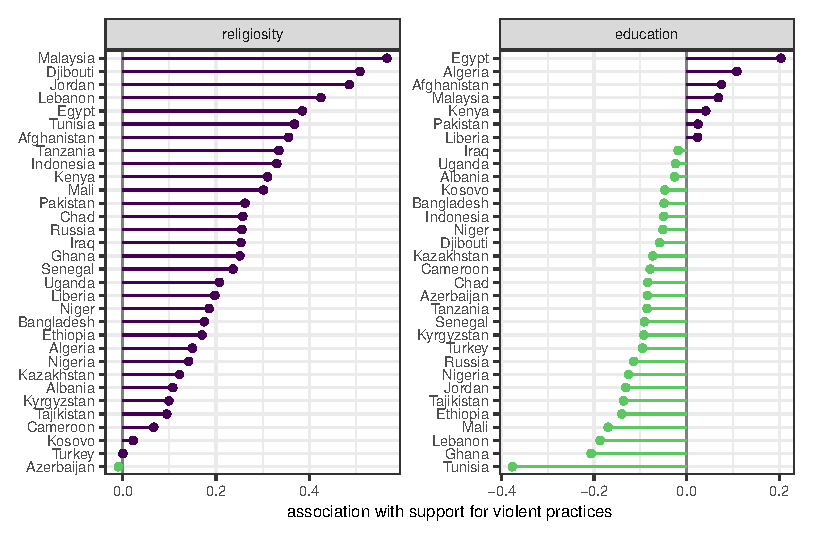
\includegraphics{figures/fig3.eps}
\caption{Lollipop plots of the association between religiosity/education
and support for violent practices in each country. Values are based on
random slopes from Model 3 of Table~\ref{tab1}. Each panel is ordered from
largest to smallest association. Values are color-coded by direction.}
\label{fig3}
%\end{adjustwidth}
\end{figure}

In contrast, all of the estimated slopes for religiosity are
consistently positive, with the exception of Azerbaijan where
religiosity effectively has no association with support for violent
practices. While the variation in these positive effects is substantial,
religiosity does not contributes substantially to lower support for
violent practices for any country within our sample.

Table~\ref{tab1} also shows the correlations between these random country
effects. Both slopes are positively related to the intercept. To explore
these correlations in more detail, Fig~\ref{fig4} shows the relationship
between the country-specific intercepts and the country-specific slopes
for religiosity and education. As Table~\ref{tab1} indicated, there is a strong
positive correlation in both cases. In countries with less support for
violent practices overall, the association between education and support
for violent practices tends to be more negative and the association
between religiosity and support for violent practices tends to be less
positive. The correlation here suggests a substantial socialization
effect on both religious and educational institutions. In more liberal
countries (those with less support for violent practices overall),
education has more of a liberalizing influence and religiosity has less
of a conservatizing influence.

\begin{figure}[!h]
%\begin{adjustwidth}{-2.25in}{0in}
\centering
%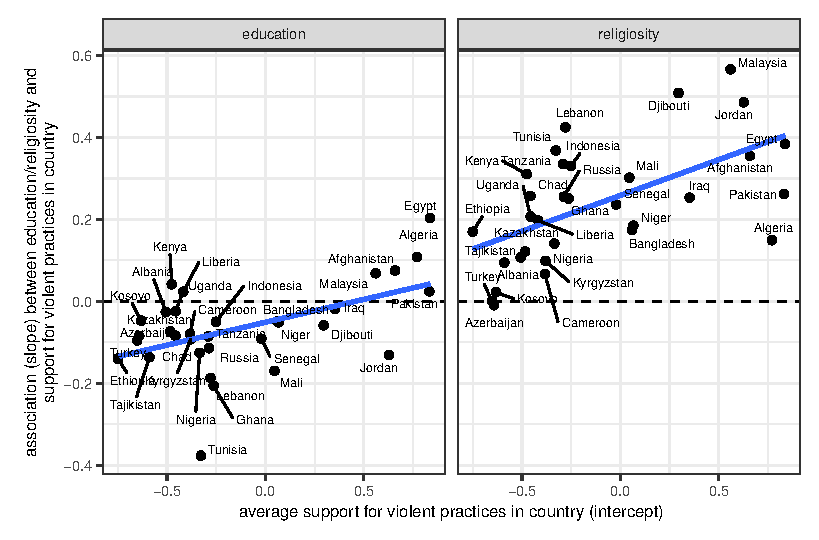
\includegraphics{figures/fig4.eps}
\caption{Scatterplot showing the relationship betwen a country's average
level of support for violent practices and the association between
education/religiosity and support for violent practices in a country.
Values are based on random intercepts and slopes from Model 3 of Table~\ref{tab1}. Best fitting OLS line is shown for both panels.}
\label{fig4}
%\end{adjustwidth}
\end{figure}

Finally, we look at the relationship between the two measures of
association. Do the effects of religiosity and education within a
country tend to work in synchronicity or are they polarized? As Table~\ref{tab1}
shows, the correlation between the two measures of association is very
low, albeit slightly positive. Figure~\ref{fig5} shows the relationship between
the two slopes on a scatterplot, confirming the low correlation. In
short, there does not seem to be any connection between educational and
religious divisions within a country on this outcome measure. For
example, Tunisia and Egypt have similar associations between religiosity
and support for violent practices, but radically different associations
between education and support for violent practices. Tunisia has by far
the most negative association of any country while Egypt has the most
positive. The results here indicate that while religiosity and education
have somewhat predictable association with support for violent
practices, the particular constellation of these two associations within
a country varies in non-predictable ways.

\begin{figure}[!h]
%\begin{adjustwidth}{-2.25in}{0in}
\centering
%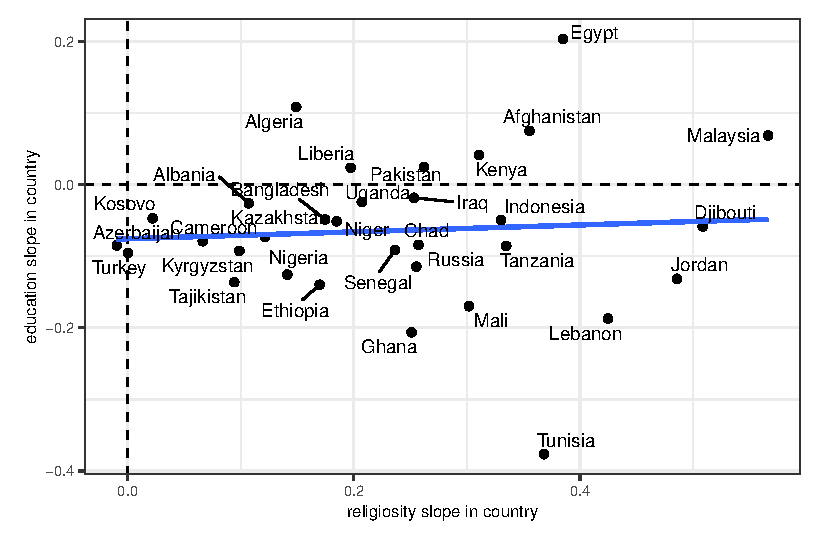
\includegraphics{figures/fig5.eps}
\caption{Scatterplot showing the relationship between country-level
associations of education and religiosity with support for violent
practices. Values based on random slopes from Model 3 of Table 1.
Best-fitting OLS line is shown.}
\label{fig5}
%\end{adjustwidth}
\end{figure}

\section*{Conclusion}

In this article, we have analyzed variation in support for violent
practices among Muslims in thirty-five countries, paying particular
attention to the effects of education, religiosity, and development on
these attitudes, as well as the heterogeneity in effects across
countries.

At first glance, the results are largely consistent with prior research
and the expectations of modernization theory. Greater development in a
country, as measured by the Human Development Index, strongly predicted
less support for violent practices. Similarly, the effects of education
and religiosity are as expected from prior research in predominantly
non-Muslim contexts, when averaged across countries. More educated
individuals are moderately less likely to support violent practices
while individuals with greater religiosity are much more likely to
support violent practices.

The association between religiosity and support for violent practices
was stronger than any other individual-level variable used in the
analysis. Importantly, this religiosity effect is not simply a surrogate
for theological conservatism or literalism. We found that while measures
of theological conservatism also predicted greater support for violent
practices, the religiosity association remains strong even after
controlling for these variables, as well as a variety of other
ideational variables.

Looking beyond the average effects across countries toward country-level
heterogeneity, the results suggest a more complex and nuanced
assessment. The effects of education and religiosity were highly
variable across countries. In a minority of countries, education
predicts more, rather than less, support for violent practices.
Similarly, in some countries there was virtually no correlation between
religiosity and support for violent practices. While we may observe
tendencies in terms of the effects of educational and religious
institutions on support for violent practices, these effects are far
from uniform and may be strongly affected by country-level
heterogeneity. In the context of the strong effect of religiosity on
support for violent practices, the heterogeneity observed here
demonstrates that there is no necessary connection between religiosity
and support for violent practices.

How can we make sense of this variation in the effects of education and
religiosity across countries? Some of this variation may reflect
idiosyncratic, historical, and path-dependent processes that are not
easily amenable to a quantitative analysis. However, we did explore two
possibilities with regard to this variation. First, we find that the
within-country association for both education and religiosity is
positively correlated with the average level of support for violent
practices in a country. In the case of education, Education exerts the
strongest negative effect on support for violent practices in countries
with the lowest average level of support overall while education has
little effect or even a positive association in countries with the most
support for violent practices overall. Religiosity has the strongest
positive effect on support for violent practices in countries with the
most support overall, and religiosity has the weakest positive effect in
countries where support for violent practices is the lowest overall.
Both findings are consistent with the socialization hypothesis, which
argues that social institutions often reflect rather than drive changes
in attitudes and values.

Second, we include the level of development as a predictor of the
association between education/religiosity and support for violent
practices. We find some evidence that the negative relationship between
education and support for violent practices is weaker in more developed
countries. This may reflect a ``flattening'' process whereby greater
development universalizes liberal values and leads to less cleavage
between educational groups. We find little evidence of an effect of
development on the association with religiosity.

As a further check on what is driving country-level heterogeneity, we
examined the correlation between the effects of religiosity and
education across countries. Somewhat surprisingly, there is very little
correlation in the effects of these two variables across countries. This
implies that there is not necessarily a greater singular force
(e.g.~``modernization'') driving change in both religious and
educational institutions, but rather that these two institutions are
affected disparately by factors unique to each country.

The heterogeneity we observe across countries places our results
somewhere between classic modernization theory and multiple modernities.
If classic modernization theory is seen as a tendency rather than a
rule, our results could be considered as an accurate reflection of its
expectations. Similarly, our results could also be seen as empirical
evidence in support of a multiple modernities approach by showing just
how different the process of modernization can be for some countries.
Nonetheless, the strong aggregate tendency toward the expectations of
classic modernization theory calls into question an unconstrained
version of the multiple modernities approach.

This heterogeneity also casts doubt on the utility of the civilizational
argument to understand value change. We find no evidence of a singular
civilizational pattern of Islamic societies. Rather, we find that the
general patterns of Islamic ``civilization'' are consistent with those
observed in non-Islamic societies but with substantial variation at the
country level. This variation cannot be explained by what is held
constant, namely Islam. We draw attention to the results for Algeria and
Tunisia to highlight this issue. Algeria and Tunisia are arguably two of
the most similar countries in our dataset by geography, language, and
culture. Yet, the observed relationships between education and support
for violent practices are not only opposite in these two countries, but
represent two of the most extreme values in the data. In Tunisia,
educational attainment strongly predicts less support for violent
practices, while in Algeria, educational attainment strongly predicts
greater support for violent practices. The implication is that we must
delve deeper into the particular historical development of each country
in order to understand this variation.

We focus in this article on whether the observed patterns in the data
are consistent with the expectations of prior theory and have attempted
to avoid the use of strong causal language throughout. Strong causal
claims are limited by the cross-sectional nature of the data. For
example, while we find that Muslims in countries with greater
development tend to have less support for violent practices, we cannot
show that a change in development is associated with a weakening of
those attitudes. Future longitudinal data would be valuable at
strengthening our understanding of causal mechanisms, albeit difficult
and costly to obtain on a sample of this size and scale.

The goal of this article has been to use statistical analysis to
leverage a large dataset and provide a birds-eye view of the
relationship between support for violent practices and individual and
country-level predictors. By necessity, this approach ignores the
specificity and nuance of country-specific historical development. Our
intent is not to discount or replace work that focuses on particular
historical cases or small N comparative/historical analyses, but rather
to complement this work with a broader comparative approach. Indeed one
of the central findings of our analysis is the substantial variation in
key relationships between countries. This suggests the possibility of
fruitful explorations at the country-level using multiple methodological
approaches to understand the substantial heterogeneity documented here.

\section*{Supporting information}

\paragraph*{S1 Appendix.}
\label{S1_Appendix}
{\bf Supplementary Materials.}  This appendix contains tables of models using alternate specifications of religiosity, education, and development.

\section*{Acknowledgments}
Cras egestas velit mauris, eu mollis turpis pellentesque sit amet. Interdum et malesuada fames ac ante ipsum primis in faucibus. Nam id pretium nisi. Sed ac quam id nisi malesuada congue. Sed interdum aliquet augue, at pellentesque quam rhoncus vitae.

\nolinenumbers

% Either type in your references using
% \begin{thebibliography}{}
% \bibitem{}
% Text
% \end{thebibliography}
%
% or
%
% Compile your BiBTeX database using our plos2015.bst
% style file and paste the contents of your .bbl file
% here. See http://journals.plos.org/plosone/s/latex for 
% step-by-step instructions.
% 
\begin{thebibliography}{10}

\bibitem{casey_real_2014}
Casey P. Real {{Time}} with {{Bill Maher}} [television broadcast]. Los Angeles; HBO; 2014 Oct 3.

\bibitem{inglehart_worldviews_2007}
Inglehart RF.
\newblock The {{Worldviews}} of {{Islamic Publics}} in {{Global Perspective}}.
\newblock In: Moaddel M, editor. Values and {{Perceptions}} of the {{Islamic}}
  and {{Middle Eastern Publics}}. {New York}: {Palgrave Macmillan US}; 2007. p.
  25--46.

\bibitem{eisenstadt_civilizational_2001}
Eisenstadt SN.
\newblock The {{Civilizational Dimension}} of {{Modernity}}: {{Modernity}} as a
  {{Distinct Civilization}}.
\newblock International Sociology. 2001;16(3):320--340.
\newblock doi:{10.1177/026858001016003005}.

\bibitem{huntington_clash_1996}
Huntington SP.
\newblock The {{Clash}} of {{Civilizations}} and the {{Remaking}} of {{World
  Order}}.
\newblock {New York}: {Simon \& Schuster}; 1996.

\bibitem{jamal_attitudes_2008}
Jamal A, Tessler M.
\newblock Attitudes in the {{Arab World}}.
\newblock Journal of Democracy; Baltimore. 2008;19(1):97--110.

\bibitem{ciftci_modernization_2010}
Ciftci S.
\newblock Modernization, {{Islam}}, or {{Social Capital}}: {{What Explains
  Attitudes Toward Democracy}} in the {{Muslim World}}?
\newblock Comparative Political Studies. 2010;43(11):1442--1470.

\bibitem{ciftci_secularislamist_2013}
Ciftci S.
\newblock Secular-{{Islamist Cleavage}}, {{Values}}, and {{Support}} for
  {{Democracy}} and {{Shari}}'a in the {{Arab World}}.
\newblock Political Research Quarterly. 2013;66(4):781--793.
\newblock doi:{10.1177/1065912912470759}.

\bibitem{mousseau_urban_2011}
Mousseau M.
\newblock Urban Poverty and Support for {{Islamist}} Terror: {{Survey}} Results
  of {{Muslims}} in Fourteen Countries.
\newblock Journal of Peace Research. 2011;48(1):35--47.
\newblock doi:{10.1177/0022343310391724}.

\bibitem{berger_foreign_2014}
Berger L.
\newblock Foreign Policies or Culture: {{What}} Shapes {{Muslim}} Public
  Opinion on Political Violence against the {{United States}}?
\newblock Journal of Peace Research. 2014;51(6):782--796.

\bibitem{inglehart_true_2003}
Inglehart R, Norris P.
\newblock The {{True Clash}} of {{Civilizations}}.
\newblock Foreign Policy. 2003;135:62--70.
\newblock doi:{10.2307/3183594}.

\bibitem{moaddel_religious_2018}
Moaddel M, Karabenick SA.
\newblock Religious {{Fundamentalism}} in {{Eight Muslim}}-{{Majority
  Countries}}: {{Reconceptualization}} and {{Assessment}}.
\newblock Journal for the Scientific Study of Religion. 2018;57(4):676--706.
\newblock doi:{10.1111/jssr.12549}.

\bibitem{jamal_reassessing_2006}
Jamal AA.
\newblock Reassessing {{Support}} for {{Islam}} and {{Democracy}} in the {{Arab
  World}}? {{Evidence}} from {{Egypt}} and {{Jordan}}.
\newblock World Affairs. 2006;169(2):51--63.

\bibitem{moaddel_introduction_2007}
Moaddel M.
\newblock Introduction: {{Theoretical}} and {{Methodological Issues}} in the
  {{Study}} of {{Values}}.
\newblock In: Moaddel M, editor. Values and {{Perceptions}} of the {{Islamic}}
  and {{Middle Eastern Publics}}. {New York}: {Palgrave Macmillan US}; 2007. p.
  1--22.

\bibitem{lerner_passing_1958}
Lerner D.
\newblock The {{Passing}} of {{Traditional Society}}: {{Modernizing}} the
  {{Middle East}}.
\newblock {New York}: {Free Press}; 1958.

\bibitem{parsons_social_1964}
Parsons T.
\newblock Social {{Structure}} and {{Personality}}.
\newblock {New York}: {Free Press}; 1964.

\bibitem{inkeles_becoming_1974}
Inkeles A, Smith DH.
\newblock Becoming {{Modern}}: {{Individual Change}} in {{Six Developing
  Countries}}.
\newblock {Cambridge, MA}: {Harvard University Press}; 1974.

\bibitem{rostow_stages_1960}
Rostow WW.
\newblock The {{Stages}} of {{Economic Growth}}: A Non-{{Communist Manifesto}}.
\newblock {Cambridge}: {Cambridge University Press}; 1960.

\bibitem{wilson_religion_1966}
Wilson BR.
\newblock Religion in {{Secular Society}}: A {{Sociological Comment}}.
\newblock {London}: {Watts}; 1966.

\bibitem{bruce_secularization_2011}
Bruce S.
\newblock Secularization: {{In Defence}} of an {{Unfashionable Theory}}.
\newblock {Oxford}: {Oxford University Press}; 2011.

\bibitem{emerson_rise_2006}
Emerson MO, Hartman D.
\newblock The {{Rise}} of {{Religious Fundamentalism}}.
\newblock Annual Review of Sociology. 2006;32(1):127--144.
\newblock doi:{10.1146/annurev.soc.32.061604.123141}.

\bibitem{scheepers_education_2002}
Scheepers P, Te~Grotenhuis M, Van Der~Slik F.
\newblock Education, {{Religiosity}} and {{Moral Attitudes}}: {{Explaining
  Cross}}-{{National Effect Differences}}.
\newblock Sociology of Religion. 2002;63(2):157--176.
\newblock doi:{10.2307/3712563}.

\bibitem{smith_future_2008}
Smith C.
\newblock Future {{Directions}} in the {{Sociology}} of {{Religion}}.
\newblock Social Forces. 2008;86(4):1561--1589.
\newblock doi:{10.1353/sof.0.0040}.

\bibitem{meyer_effects_1977}
Meyer JW.
\newblock The {{Effects}} of {{Education}} as an {{Institution}}.
\newblock American Journal of Sociology. 1977;83(1):55--77.
\newblock doi:{10.1086/226506}.

\bibitem{chabbott_development_2000}
Chabbott C, Ramirez FO.
\newblock Development and {{Education}}.
\newblock In: Hallinan MT, editor. Handbook of the {{Sociology}} of
  {{Education}}. Handbooks of {{Sociology}} and {{Social Research}}. {Boston,
  MA}: {Springer US}; 2000. p. 163--187.

\bibitem{depaepe_educationalization_2008}
Depaepe M, Smeyers P.
\newblock Educationalization as an {{Ongoing Modernization Process}}.
\newblock Educational Theory. 2008;58(4):379--389.

\bibitem{hyman_education_1979}
Hyman HH, Wright CR.
\newblock Education's {{Lasting Influence}} on {{Values}}.
\newblock {Chicago, IL}: {University of Chicago Press}; 1979.

\bibitem{bobo_education_1989}
Bobo L, Licari FC.
\newblock Education and {{Political Tolerance}}: {{Testing}} the {{Effects}} of
  {{Cognitive Sophistication}} and {{Target Group Affect}}.
\newblock The Public Opinion Quarterly. 1989;53(3):285--308.

\bibitem{weakliem_effects_2002}
Weakliem DL.
\newblock The {{Effects}} of {{Education}} on {{Political Opinions}}: {{An
  International Study}}.
\newblock International Journal of Public Opinion Research.
  2002;14(2):141--157.
\newblock doi:{10.1093/ijpor/14.2.141}.

\bibitem{kingston_why_2003}
Kingston PW, Hubbard R, Lapp B, Schroeder P, Wilson J.
\newblock Why {{Education Matters}}.
\newblock Sociology of Education. 2003;76(1):53--70.
\newblock doi:{10.2307/3090261}.

\bibitem{adorno_authoritarian_1950}
Adorno TW.
\newblock The {{Authoritarian Personality}}.
\newblock {New York}: {Harper}; 1950.

\bibitem{mcclosky_dimensions_1983}
Mcclosky H, Brill A.
\newblock The {{Dimensions}} of {{Tolerance}}: {{What Americans Believe About
  Civil Liberties}}.
\newblock {New York}: {Russell Sage Foundation}; 1983.

\bibitem{selznick_tenacity_1969}
Selznick GJ, Steinberg S.
\newblock The {{Tenacity}} of {{Prejudice}}: Anti-{{Semitism}} in
  {{Contemporary America}}.
\newblock {New York}: {Harper \& Row}; 1969.

\bibitem{jackman_education_1984}
Jackman MR, Muha MJ.
\newblock Education and {{Intergroup Attitudes}}: {{Moral Enligtenment}},
  {{Superficial Democratic Commitment}} or {{Ideological Refinement}}?
\newblock American Sociological Review. 1984;49:751--769.

\bibitem{phelan_education_1995}
Phelan J, Link BG, Stueve A, Moore RE.
\newblock Education, {{Social Liberalism}}, and {{Economic Conservatism}}:
  {{Attitudes Toward Homeless People}}.
\newblock American Sociological Review. 1995;60(1):126--140.
\newblock doi:{10.2307/2096349}.

\bibitem{weil_variable_1985}
Weil FD.
\newblock The {{Variable Effects}} of {{Education}} on {{Liberal Attitudes}}:
  {{A Comparative}}- {{Historical Analysis}} of {{Anti}}-{{Semitism Using
  Public Opinion Survey Data}}.
\newblock American Sociological Review. 1985;50(4):458--474.
\newblock doi:{10.2307/2095433}.

\bibitem{schwadel_explaining_2015}
Schwadel P.
\newblock Explaining {{Cross}}-{{National Variation}} in the {{Effect}} of
  {{Higher Education}} on {{Religiosity}}.
\newblock Journal for the Scientific Study of Religion. 2015;54(2):402--418.
\newblock doi:{10.1111/jssr.12187}.

\bibitem{rokeach_part_1969}
Rokeach M.
\newblock Part {{I}}. {{Value Systems}} in {{Religion}}.
\newblock Review of Religious Research. 1969;11(1):3--23.
\newblock doi:{10.2307/3510550}.

\bibitem{rokeach_part_1969a}
Rokeach M.
\newblock Part {{II}}. {{Religious Values}} and {{Social Compassion}}.
\newblock Review of Religious Research. 1969;11(1):24--39.
\newblock doi:{10.2307/3510551}.

\bibitem{wilcox_evangelicals_1990}
Wilcox C, Jelen T.
\newblock Evangelicals and {{Political Tolerance}}.
\newblock American Politics Quarterly. 1990;18(1):25--46.
\newblock doi:{10.1177/1532673X9001800102}.

\bibitem{kelley_class_1995}
Kelley J, Evans MDR.
\newblock Class and {{Class Conflict}} in {{Six Western Nations}}.
\newblock American Sociological Review. 1995;60(2):157--178.
\newblock doi:{10.2307/2096382}.

\bibitem{scheepers_religion_1998}
Scheepers P, Van Der~Slik F.
\newblock Religion and {{Attitudes}} on {{Moral Issues}}: {{Effects}} of
  {{Individual}}, {{Spouse}} and {{Parental Characteristics}}.
\newblock Journal for the Scientific Study of Religion. 1998;37(4):678--691.
\newblock doi:{10.2307/1388149}.

\bibitem{karpov_religiosity_2002}
Karpov V.
\newblock Religiosity and {{Tolerance}} in the {{United States}} and
  {{Poland}}.
\newblock Journal for the Scientific Study of Religion. 2002;41(2):267--288.
\newblock doi:{10.1111/1468-5906.00116}.

\bibitem{norris_sacred_2011}
Norris P, Inglehart R.
\newblock Sacred and {{Secular}}: {{Religion}} and {{Politics Worldwide}}.
\newblock {Cambridge}: {Cambridge University Press}; 2011.

\bibitem{kelley_national_1997}
Kelley J, De~Graaf ND.
\newblock National {{Context}}, {{Parental Socialization}}, and {{Religious
  Belief}}: {{Results}} from 15 {{Nations}}.
\newblock American Sociological Review. 1997;62(4):639--659.
\newblock doi:{10.2307/2657431}.

\bibitem{fukuyama_end_1992}
Fukuyama F.
\newblock The {{End}} of {{History}} and {{The Last Man}}.
\newblock {New York}: {Free Press}; 1992.

\bibitem{hefner_multiple_1998}
Hefner RW.
\newblock Multiple {{Modernities}}: {{Christianity}}, {{Islam}}, and
  {{Hinduism}} in a {{Globalizing Age}}.
\newblock Annual Review of Anthropology. 1998;27:83--104.

\bibitem{eisenstadt_multiple_2000}
Eisenstadt SN.
\newblock Multiple {{Modernities}}.
\newblock Daedalus. 2000;129(1):1--29.

\bibitem{kamali_multiple_2006}
Kamali M.
\newblock Multiple {{Modernities}}, {{Civil Society}} and {{Islam}}: The
  {{Case}} of {{Iran}} and {{Turkey}}.
\newblock {Liverpool}: {Liverpool University Press}; 2006.

\bibitem{casanova_cosmopolitanism_2011}
Casanova J.
\newblock Cosmopolitanism, {{The Clash}} of {{Civilizations}} and {{Multiple
  Modernities}}.
\newblock Current Sociology. 2011;59(2):252--267.
\newblock doi:{10.1177/0011392110391162}.

\bibitem{pewforumonreligionandpubliclife_global_2012}
{Pew Forum on Religion and Public Life}. The {{Global Religious Landscape}};
  2012.

\bibitem{glock_religion_1965}
Glock CY, Stark R.
\newblock Religion and {{Society}} in {{Tension}}.
\newblock {Chicago}: {Rand McNally}; 1965.

\bibitem{el-menouar_five_2014}
{El-Menouar} Y.
\newblock The Five Dimensions of {{Muslim}} Religiosity. {{Results}} of an
  Empirical Study.
\newblock methods, data, analyses. 2014;8(1):26.

\bibitem{buuren_mice_2011}
van Buuren S, {Groothuis-Oudshoorn} K.
\newblock {{MICE}} : {{Multivariate Imputation}} by {{Chained Equations}} in
  {{R}}.
\newblock Journal of Statistical Software. 2011;45(3).
\newblock doi:{10.18637/jss.v045.i03}.

\bibitem{gelman_scaling_2008}
Gelman A.
\newblock Scaling {{Regression Inputs}} by {{Dividing}} by {{Two Standard
  Deviations}}.
\newblock Statistics in Medicine. 2008;27(15):2865--2873.
\newblock doi:{10.1002/sim.3107}.

\end{thebibliography}

%\bibliography{../../project.bib}

\end{document}
